\documentclass[acmlarge,screen=false,language=chinese,language=english]{acmart}
\usepackage[utf8]{inputenc} % allow utf-8 input
\usepackage[T1]{fontenc}    % use 8-bit T1 fonts
\usepackage{hyperref}       % hyperlinks
\usepackage{url}            % simple URL typesetting
\usepackage{booktabs}       % professional-quality tables
\usepackage{amsfonts}       % blackboard math symbols
\usepackage{nicefrac}       % compact symbols for 1/2, etc.
\usepackage{microtype}      % microtypography
\usepackage{xcolor}         % colors
\usepackage{multirow}
\usepackage{graphicx}
\usepackage{subcaption}
\usepackage{tikz}
\usetikzlibrary{shapes.geometric}
\usetikzlibrary{decorations.pathreplacing,calligraphy}
\usetikzlibrary{positioning}
\usetikzlibrary{arrows.meta}

\usepackage{gbt7714}
\usepackage{xeCJK}
\setCJKmainfont{SimSun}
\newCJKfontfamily[hei]\myhei{SimHei}
\bibliographystyle{gbt7714-numerical}

\bibpunct{[}{]}{,}{n}{}{;}
\setcitestyle{numbers, square}
\newcommand{\thickhline}{\hline}

\title{LLMs for Software Supply Chain Security: Boon or Bane?}
\translatedtitle{chinese}{\myhei 大语言模型之于软件供应链安全: 利与弊}

\begin{CCSXML}
<ccs2012>
   <concept>
       <concept_id>10002978.10003022.10003023</concept_id>
       <concept_desc>Security and privacy~Software security engineering</concept_desc>
       <concept_significance>500</concept_significance>
       </concept>
 </ccs2012>
\end{CCSXML}

\ccsdesc[500]{Security and privacy~Software security engineering}

\keywords{Large Language Model, Software Supply Chain, AI Governance}
\translatedkeywords{chinese}{大语言模型, 软件供应链, 人工智能治理}

\author{Rundong Yang}
\orcid{0009-0003-6567-7741}
\email{22307140045@m.fudan.edu.cn}
\affiliation{
\institution{Fudan University}
\department{College of Computer Science and Artificial Intelligence}
\city{Shanghai}
\country{China}
}
\settopmatter{printacmref=false, printccs=true, printfolios=false}
\setcopyright{none}
\setcctype{zero}
\acmArticleType{Review}
\acmDataLink{https://github.com/Fudanyrd/llm4ssc}

% FORGED
\acmDOI{10.1145/5555555-aaaaaaa}
\acmISBN{aaaa-5555}
\acmVolume{9}
\acmNumber{4}
\acmArticle{25}
\acmYear{2026}
\acmJournal{CSUR}

\begin{document}
\begin{abstract}
  %\par {~}
  \begin{tabular}{p{\linewidth}}
\textbf{Background:} the Software Supply Chain has become a critical
digital infrastructure. Although the attack and defense techniques of
Software Supply Chain is researched extensively, the Large Language
Models' implications for its safety and security are yet to
be examined.

\\

\textbf{Method:} to this end, we conducted a Systematic Literature
Review covering 81 "LLM for Software Supply Chain" studies published
in the past 5 years across 4 databases. This enables us to understand both
LLM-based defense techniques and potential attack surfaces.
The artifact of our literature review can be found at 
\url{https://github.com/Fudanyrd/llm4ssc}.

\\

\textbf{Results:} based on our literature review and
quantitative analysis,
we conclude that the majority of defense/attack techniques
operate on the source code and compiled artifacts, whereas the
study of attacking/defending build infrastructures and  human
developers is lagging. We also suggested methods to mitigate
LLM-based attacks at the end, calling for ethical and responsible
use of LLM in software development and shedding light on
AI governance.


\end{tabular}


\end{abstract}

\maketitle
\section{Introduction}\label{sec:intro}

%^C In one paragraph: introduce Software Supply Chain.
%^C How vital is it? (accelerate development; provide usable components)
%^C How severely has it been compromised?
%^C List examples of SSC attacks (xz-utils, log4j)
\par The Software Supply Chain (SSC) lies at the basis of modern digital
infrastructure. By providing software developers with reusable libraries,
packages, or components which can be assembled into a larger software
project\citep{sscdirection}, Software Supply Chain is integral to boosting
development efficacy, improving software quality, and reduce development cost
\citep{brooks1987no,mythicalmanmonth}. However, the number of Software Supply
Chain attacks, which come in the form of ransomware, backdoor, or vulnerability
injected into the source code, has grown exponentially over recent years.
This can be evidenced by the surging number of Common Vulnerabilities and
Exposures (CVEs), indicating the wide susceptibility of softwares. Also
Sonatype, a software supply chain platform, observed an annual increase of 156\%
in number of malicious packages, reaching a startling number of 704,102 identified
since 2019 \citep{sonatype2024report}. Such proliferation of malicious or
vulnerable components, coupled with exploding consumption of open-source 
packages and failure to promptly respond to reported vulnerabilities such as CVEs 
\citep{sonatype2024report}, have made Software Supply Chain
a broad attack surface, bringing about data or financial loss to
affected software developers and users.
For instance, the \texttt{xz-util} incident is an example of deliberately
injected backdoor, allowing the attacker to intercept sensitive data
or gain control of the affected machine \citep{xzincident}.
Despite all on-going efforts for security 
assurance and attack detection (e.g. \citep{konala25metadata,11022932,10695665}),
the sheer volume of risk to the
security of Software Supply Chain calls for new methods of governance.

%^C Introduce Large language model, in a more general way.
\par Recent advancements in Large Language Models (LLMs), including
improvement in model's intrinsic
capabilities\citep{llmsurvey,overviewllm,csllm} and the innovations of
enhancement techniques, contributed to their active involvement in
software engineering tasks, such as code suggestion, code completion, and
code review \citep{llm4se, llm4se2}. Because of their contextual reasoning
capacities and understanding of code intent, several studies have
explored leveraging these language models for guarding the security
of Software Supply Chain. For instance, by means of 
\textit{threat detection} (e.g. \citep{llmbackdoordet,singla2023empiricalstudyusinglarge,syed2025agenticaiautonomousdefense}),
malicious code such as backdoors in software packages can be 
reported; through enhanced \textit{security testing} and \textit{vulnerability detection}
(e.g. \citep{11022932,10695665,10628694}), vulnerabilities 
can be uncovered before exploitation; via automated \textit{vulnerability repair}
(e.g. \citep{vulrepairusingllm,vulmaster}), attackers have less time and chance
to exploit a reported vulnerability. LLM for Software Supply Chain
defense techniques will be discussed in Section~\ref{sec:rq2}.

\par Nevertheless, Large Language Models may be used equally for the good
and the evil. LLMs are susceptible to both intrinsic hallucinations and
a wide variety of attacks. Section~\ref{sec:rq3} discusses LLM's potential
of generating code with vague vulnerabilities or malice, because
of either internal hallucinations or deliberate attack on its
training data and prediction process. Furthermore, LLM's capability of
generating readable text has been leveraged for social engineering attack,
such as crafting phishing emails.

\par To the best of our knowledge, this study is the first to examine the
Large Language Model's implications of the security of Software Supply Chain.
It makes the following contributions:

\begin{itemize}
  \item A systematic literature review of LLM-based
  Software Supply Chain defense techniques (Section~\ref{sec:rq2}).

  \item A rigorous analysis of LLM's vulnerabilities and possible
  exploitations of LLM in Software Supply Chain attacks, in Section~\ref{sec:rq3}.

  \item Insights into mitigation of LLM-assisted Software Supply Chain
  attacks. They serve as guidance to responsible, ethical, and non-malignant
  use of LLM in Software Supply Chain.
\end{itemize}


\section{Methodology}\label{sec:method}

This study adopts Systematic Literature Review (SLR) methodology for 
identifying relevant studies and research gaps. This SLR follows 
guidance provided by B. Kitchenham et al. \citep{segress} and
S. Keele et al. \citep{slrguidese}, and incorporates three major
steps: \textbf{Planning the Search} (\ref{subsec:search}), 
\textbf{Study Selection} (\ref{subsec:stusel}),
and \textbf{Data Analysis}.

\subsection{Search Strategy}\label{subsec:search}

As shown in Figure~\ref{fig:stusel},
we employed \textbf{Precise Search Strategy} \citep{optimalsearch}
for article search, i.e., 
we crafted the search string to maximize the relevance 
of resulting studies. More specifically, we followed the following three steps
in order to establish a set of relevant studies:


\begin{enumerate}
 \item Conduct an automated search of studies published within 5 years
  (i.e. after 2022)  based on our crafted search string;
 \item Screen the title and abstract of all articles and filter by
       inclusion/exclusion criteria;
 \item Conduct snowballing search on the result of previous step.
\end{enumerate}

\begin{figure}[ht]

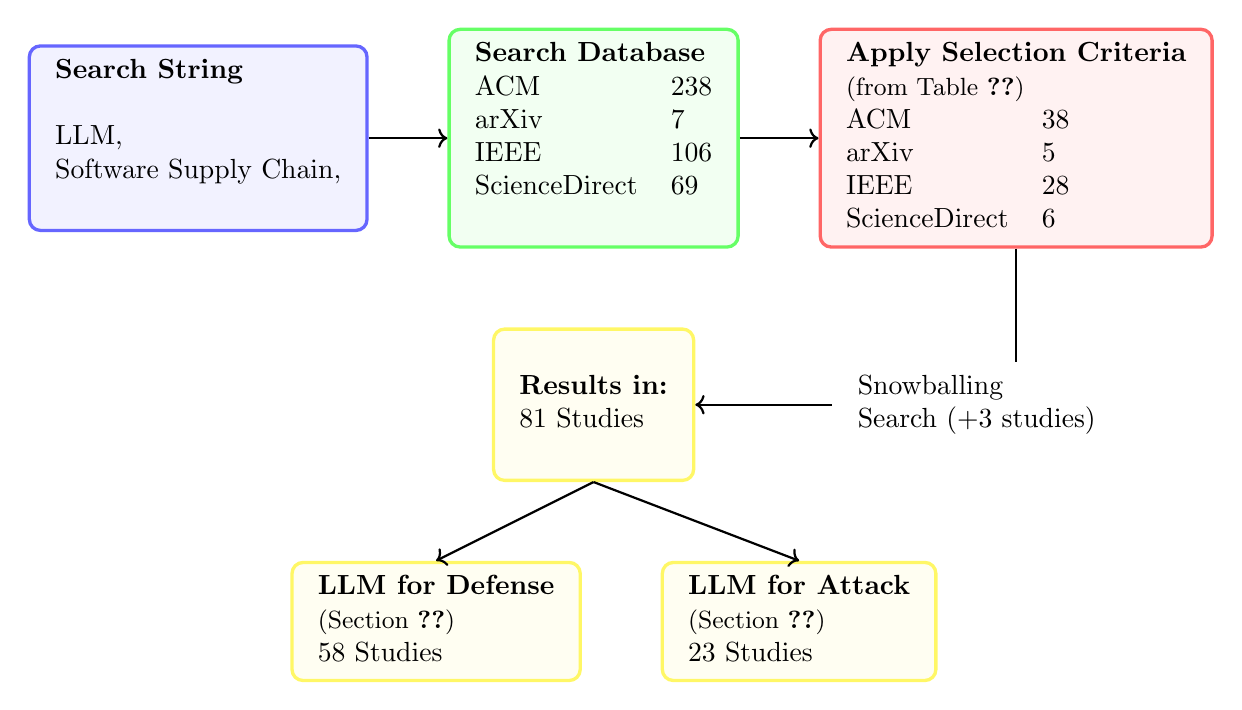
\begin{tikzpicture}[
  every node/.style={fill=white},
  str/.style={rectangle, rounded corners, draw=blue!60, fill=blue!5, very thick, minimum size=10mm},
  db/.style={rectangle, rounded corners, draw=green!60, fill=green!5, very thick, minimum size=10mm},
  filt/.style={rectangle, rounded corners, draw=red!60, fill=red!5, very thick, minimum size=10mm},
  res/.style={rectangle, rounded corners, draw=yellow!60, fill=yellow!5, very thick, minimum size=10mm},
]

  \node[str] (sstr) {
    \begin{tabular} {l}
      \textbf{Search String} \\
       \\
      LLM, \\
      Software Supply Chain, \\
      \\
    \end{tabular}
  };

  \node[db] (sdb) [right=of sstr] {
    \begin{tabular} {ll}
      \multicolumn{2}{l}{\textbf{Search Database}}\\
      ACM & 238 \\
      arXiv & 7 \\
      IEEE & 106 \\
      ScienceDirect & 69 \\
      & \\
    \end{tabular}
  };


  \node[filt] (sfilt) [right=of sdb] {
    \begin{tabular} {ll}
      \multicolumn{2}{l}{\textbf{Apply Selection Criteria}}\\
      \multicolumn{2}{l}{\small (from Table~\ref{tab:criteria})} \\
      ACM & 38 \\
      arXiv & 5 \\
      IEEE & 28 \\
      ScienceDirect & 6 \\
    \end{tabular}
  };

  \node[res] (result) [below=of sdb] {
    \begin{tabular}{l}
      \\
      \textbf{Results in:} \\
      81 Studies \\
      \\
    \end{tabular}
  };

  \node[res] (defense) [below=of result, xshift=-2cm] {
    \begin{tabular}{l}
      \textbf{LLM for Defense} \\
      {\small (Section~\ref{sec:rq2})} \\
      58 Studies \\
    \end{tabular}
  };

  \node[res] (attack) [right=of defense] {
    \begin{tabular}{l}
      \textbf{LLM for Attack} \\
      {\small (Section~\ref{sec:rq3})} \\
      23 Studies \\
    \end{tabular}
  };

  \draw [thick, ->] (sstr.east) -- (sdb.west);
  \draw [thick, ->] (sdb.east) -- (sfilt.west);
  \draw [thick, ->] (sfilt.south) |- node[xshift=-0.5cm] {
    \begin{tabular}{l}
    Snowballing \\
    Search (+3 studies) \\
    \end{tabular}
  } (result.east);
  \draw[thick, ->] (result.south) -- (defense.north);
  \draw[thick, ->] (result.south) -- (attack.north);
\end{tikzpicture}

\caption{The process of study identification and selection.}
\label{fig:stusel}
\end{figure}

\par Our search string needs to combine two sets of keywords, one related
to Software Supply Chain, the other concerned about Large Language Models.
For automated search, intra-set keywords are OR-ed, and inter-set keywords
are AND-ed to form the final search string.
The complete set of keywords are as follows:

\begin{itemize}
  \item \textit{Phrases related to Software Supply Chain}: supply chain, software.

  \item \textit{Phrases related to LLMs}: language model, agent.

  \item \textit{Phrases of task definition}: attack, breach, defend, detect, vulnerability.
\end{itemize}

\par It is important to note that the list of keywords related to 
LLMS we setup includes \textit{agent}, that does not seem to be
necessarily related to LLMs. The reason for this is that we observe 
recent prevalence in LLM-based agentic technologies \citep{agents} (the technique
behind many AI assistant, such as OpenClaw and \texttt{opencode}) ,
and that we want to avoid omitting
articles related to our research as much as possible.

\paragraph*{Search Databases.} After determining the search strings, we
employed the SLR Tool\citep{slrtool} and conducted
an automated search across four widely used databases
\footnote{ACM Digital Library, arXiv, IEEE Xplore, Science Direct}, 
which cover most published
articles and preprints of under-review articles. Given that the first
LLM trained on code corpus was published in 2021\citep{codex}, 
we focus our search on articles
published from that year onward. The search results from each database were
merged and deduplicated with SLR Tool\citep{slrtool}.
As a result, we obtained 238 articles from ACM Digital Library, 
7 articles from arXiv, 106 articles from IEEE Xplore, 
and 69 articles from Science Direct.

\subsection{Study Selection}\label{subsec:stusel}

\par Using our search strategy, we initially obtained 420 articles
that potentially relate to our research. Next, we further 
evaluate the relevance of these articles based on our inclusion
and exclusion criteria, as shown in Table~\ref{tab:criteria}.
Unlike previous SLRs \citep{llm4se2}, we do not exclude papers
published in workshop track, because their reference lists
may benefit our snowballing search.
In this step, we conducted a manual selection by examining the 
title, abstract, and keywords of each article, resulting
in a total of 81 papers.

\begin{table}[ht]
  \centering
  \caption{Inclusion and Exclusion Criteria for Study Selection}
  \label{tab:criteria}
\begin{tabular}{ll}
\thickhline
\multicolumn{2}{c}{\textbf{Inclusion Criteria}} \\ \hline
    (1) & The study claims an LLM is used. \\
    (2) & The study involves Software Supply Chain. \\
    (3) & The study is full-text available. \\
     & \\
\thickhline
\multicolumn{2}{c}{\textbf{Exclusion Criteria}} \\ \hline
    (1) & The study is concerned with LLM supply chain. \\
    (2) & Non-English written literature. \\
    (3) & Tool demos and editorials; \\
     & \\
\thickhline
\thickhline
\end{tabular}
\end{table}

\paragraph*{Snowballing Search}
To identify any additional 
 possibly relevant primary studies, we conducted a snowballing 
 search. Snowballing search refers to using the reference list
 of an article or the citations to the article to identify additional
 articles (which must also comply with our
 selection criteria shown in Table~\ref{tab:criteria}). 
As a result, we obtained an additional 3 studies.




% Body: research questions.
\section{RQ1 -- LLM Optimization for Software}\label{sec:rq1}

\par This Research Question studies how LLMs are enhanced and optimized
for software
engineering tasks, which aims to provide necessary background knowledge
for later sections. We anticipate that these LLM-enhancement techniques
can be equally generalized to Software Supply Chain tasks, because both
kinds of tasks involve code comprehension and code summary. 

\par This RQ is conducted by a case-study of \texttt{opencode},
followed by a
brief literature review of collected LLM-enhancement techniques.
\texttt{opencode} is "an open source AI coding agent" capable of
a series of software engineering tasks, such as code completion,
code review, and code summary \citep{opencode}. The case-study
of \texttt{opencode}'s internal implementation helps us identify 
the enhancement techniques for this RQ: \textit{Prompting}\citep{promptsurvey} 
and \textit{Agentic Framework}\citep{agents,agentsurvey}.
Other techniques include \textit{Retrieval Augmented Generation}
(RAG) \citep{ragsurvey} and \textit{Fine-tuning}, both of which have 
limited flexibility and will not be discussed.

\paragraph*{Prompt Engineering} Also known as \textit{prompting},
this technique tunes the Large Language Model's input (the prompt)
to boost performance. Common kinds of prompting
techniques include zero
shot learning \citep{zeroshot1, zeroshot2} (update the prompt
for multiple rounds and observe LLM's performance), few
shot learning \citep{fewshot1, fewshotlearner} (provide
a few examples of expected answer)
and/or chain-of-thought \citep{cotprompt}
prompting (CoT, explicitly ask the LLM to show its reasoning process
), as well as their variants.
In practice, these prompts are loaded on-demand by the user,
via a group of text files known as \textit{Plugins} 
(\texttt{opencode} terminology) and \textit{Skills}
(\texttt{OpenClaw}\citep{openclaw} terminology).
By providing helpful contexts including task definition ("What to achieve")
instructions ("How to achieve"), these media of prompts
are helping LLMs yield better outcomes, and have become
a crucial part of today's AI ecosystem (also part of
Software Supply Chain).

\paragraph*{Agentic Framework} It is also known as \textit{harness engineering}
(a term that seems to be defined as the construction of
agent's execution infrastructure \citep{harnessengineeringalgorithm}.).
The objective of agentic framework is to equip the Large Language Model
with the ability to explore its surrounding \textit{environment},
to execute actions, and to keep memory of its context.
With such autonomous execution capability,
agentic frameworks such as \texttt{opencode} free software developers
from the tedious task of turning the idea or requirement into
executable source code.

\par From the documentation of \texttt{opencode}\citep{opencode},
we are able to build a mental model of the architecture of LLM-based
agents, as shown in Figure~\ref{fig:agentarch}.

\begin{figure}[ht]
	\centering
	\begin{tikzpicture}[
         every node/.style={fill=white},
		llm/.style={rectangle, rounded corners, draw=blue!60, fill=blue!5, very thick, minimum size=5mm},
        prompt/.style={rectangle, rounded corners, draw=green!60, fill=green!5, very thick, minimum size=5mm},
        others/.style={rectangle, rounded corners, draw=red!60, fill=red!5, very thick, minimum size=5mm},
    ]

		\node[llm, align=left] (lm) {
			\par 
\includegraphics[width=2cm]{logo/llm.png}
			\par ~LLM~
		};

		\node[others, align = center] (parser) [left=of lm, xshift=-2cm] {
			\begin{tabular}{l}
                \makebox[2.5cm][c]{Response Parsing} \\
				
\includegraphics[width=2.5cm]{logo/parsing.png}
			\end{tabular}
		};

		\node[prompt] (prompt) [right=of lm] {
			\begin{tabular}{l}
                \makebox[2cm][c]{Prompt} \\
                
\includegraphics[width=2cm]{logo/prompt.png}
            \end{tabular}
		};

        \node[others] (tool) [below=of lm] {
			\par 
\includegraphics[width=2cm]{logo/tool.png}
            \par ~Tool~
        };
        \node[others] (mem) [above=of lm] {
            \par 
\includegraphics[width=2cm]{logo/memory.png}
            \par Memory
        };

        \draw[thick, ->] (lm) -- node[]
                    {generate} (parser);
        \draw[thick, ->] (prompt) -- (lm);
		\draw[thick, ->] (parser.south) |- node[xshift=1cm]
									{Invoke} 
									(tool.west);
		\draw[thick, ->] (parser.north) |- node[xshift=1cm]
									{Update}
									(mem.west);
		% memory --(Task Description, Plan, ...) --> prompt
        \draw[thick, ->] (mem) -| node[xshift=1cm]
                    {Task Description, Prompt Plugins} 
                    (prompt);
	    % tool --(output filtering/summarizing) --> prompt
        \draw[thick, ->] (tool) -| node[xshift=1cm]
                    {output filtering/summarizing} 
                    (prompt);
		% memory --(RAG) --> llm
        \draw[dotted, ->] (mem) -| node[yshift=-1.5cm]
                    {MCP} 
                    (lm);
    \end{tikzpicture}

    \caption{Typical Architecture of LLM-based agents.}
    \label{fig:agentarch}
\end{figure}

\begin{itemize}
 \item \textbf{A tool set}, usually consisting of file editor, 
   command executor (e.g. the shell), 
   and language server \footnote{useful for code completion and go-to definition}.
  It is the tools that enable the agent to autonomously interact with
  the execution environment and complete task on behalf of user.

 \item A \textbf{memory module} providing essential task contexts,
  including task definition, project documentation, and 
  suggesting next action for the LLM.
  Also, the LLM can dynamically update (refine) the content of memory.
  The memory is useful for resuming previously interrupted tasks
  (without starting from scratch).

 \item \textbf{The Large Language Model}, which serves as the foundation 
  of the agent, generates responses based on the
  prompt and the contexts provided by the memory module, and then
  invokes tools based on the generated response.

 \item A \textbf{Response Parser} is used to parse the LLM's 
     response and determine the next action, which can be either 
     invoking a tool or updating the memory module.

 \item Occasionally \textbf{MCP Server}. The Model Context Protocol
 (MCP) aims to provide a unified and open standard for exchanging
 data between the LLM-based agent and its execution environment,
  thereby improving simplicity and reliability \citep{mcpintro}.
 For the benefits of this protocol, the LLM-based agent
  can safely access remote data source (managed by MCP server)
  via tool invocation (i.e. the agent is an MCP client).
 
\end{itemize}


\paragraph*{RQ1 -- Summary}

\begin{itemize}
  \item This RQ began with a case-study with \texttt{opencode}
  \citep{opencode}, from which a set of LLM optimization
  techniques are identified -- \textit{Prompting} and
  \textit{Agentic Framework}.

  \item This RQ laid the foundation for later sections.
  Through the study of the ecosystem of LLM-based
  agents, their security weaknesses can be discussed.
\end{itemize}



\section{RQ2: In what ways are LLMs employed to secure SSC?}
\label{sec:rq2}

\par This Research Question examines how LLM defend Software Supply Chain
security, by means of reviewing collected literature. We begin by 
introducing the major attack vectors of SSC breaches, and then review
how LLMs are leveraged to mitigate these kinds of attacks. 

% IMPORTANT NOTE: this is not my original work.
\paragraph*{What are the attack vectors against SSC?} L. Williams et al.
categorized the three major attack vectors as follows\citep{sscdirection}:


% these are my words, i.e. paraphrased.
\begin{itemize}
  \item (Vector 1) Through malwares or vulnerabilities injected into open-source packages/libraries
  and other third-party dependencies (e.g. the \texttt{xz-util} incident 
  \citep{xzincident});

  \item (Vector 2) Through compromising the build infrastructure (e.g. CI/CD) where the
  software component is tested, packed and deployed;

  \item (Vector 3) Through targeting human developers involved in software development,
  such as \textit{Social Engineering}.
\end{itemize}

% Generated from dataset/rq2.json
\begin{figure}[ht]
  \centering
  \subcaptionbox{Distribution by year.}
    {\includegraphics[width=0.45\textwidth]{logo/rq2trend.pdf}}
  \subcaptionbox{Distribution by attack vectors.}
    {\includegraphics[width=0.45\textwidth]{logo/rq2dist.pdf}}

  \caption{Distribution of LLM-based Mitigation Publications.}
  \label{fig:rq2dist}
\end{figure}

\paragraph*{Trend Analysis.} The distributions of publications over
different types of attack vectors and year are shown in Figure~\ref{fig:rq2dist}.
We observe that defending Software Supply Chain against \textit{attack vector 1} is
steadily on the rise, with only few exceptions where defense to \textit{attack vector 2}
is studied. Apart from a few surveys in which \textit{attack vector 3} is introduced
(e.g. \cite{sscdirection}), we have found no studies proposing defense to
this kind of SSC attack.

% Generated from dataset/domain.json
% "package manager" : e.g. npm, maven, PyPI, etc.
% "AI Model" (platform) e.g. HuggingFace and application (e.g. LLM-integrated app
% \cite{10.1145/3756681.3757083})
% "Agent harness" includes Skills, plugins, MCP, etc.
\paragraph*{Which components of Software Supply Chain are secured by LLM?}

\subsection{Mitigation of Malware and Vulnerabilities}\label{subsec:vec1}


\begin{figure}[ht]
  \centering
  \includegraphics[width=\textwidth]{logo/vec1taxo.pdf}

  \caption{Taxonomy of Attack Vector 1 Mitigation Techniques. \\
   {\small \textit{det.} is short for the word detection; \textit{lib.} is short for the word library.} \\
   {\small Enclosure of circles implies logical enclosure; the size of circle
   is roughly proportional to \# studies obtained.}
  }
\end{figure}

\subsection{Mitigation of Build System Vulnerabilities}\label{subsec:vec2}



\section{RQ3 -- Potential SSC Risks Imposed by LLM}
\label{sec:rq3}

\par As shown in Figure~\ref{fig:llmrisk},
 we summarized possible vulnerabilities  of an LLM, which
 may posit attack surfaces to the Software Supply Chain,
 across its lifecycle --
\textit{training \& tuning} stage, \textit{inference} stage,
and \textit{agent} stage.  This section then
delves into how these vulnerabilities turn against
Software Supply Chain security.

\begin{figure}
  % \documentclass{standalone}
% \usepackage{tikz}
% \usepackage{multirow}
% \usetikzlibrary{shapes.geometric}
% \usetikzlibrary{decorations.pathreplacing,calligraphy}
% \usetikzlibrary{positioning}
% \usetikzlibrary{arrows.meta}
% \begin{document}

\begin{tikzpicture}[
  every node/.style={fill=white},
  base/.style={rectangle, rounded corners, draw=blue!60, fill=blue!5, very thick, minimum size=2.5cm},
  sys/.style={rectangle, rounded corners, draw=green!60, fill=green!5, very thick, minimum size=2.5cm},
  vuln/.style={rectangle, rounded corners, draw=red!60, fill=red!5, very thick, minimum size=2.5cm},
]


\node[base] (tt) {
\begin{tabular}{cc}
  \multicolumn{2}{c}{\textbf{Training \& Tuning}} \\
  \begin{tikzpicture}[
  vuln/.style={rectangle, rounded corners, draw=red!60, fill=red!5, very thick},
  ]
 \node [vuln] (v) {
    \begin{tabular}{c}
    \makebox[2cm][c]{\small Data Poisoning} \\
    \cite{11344010,11028470}
    \end{tabular}
 };
  \end{tikzpicture} &
  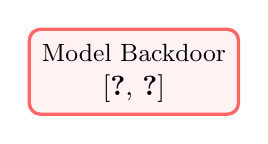
\begin{tikzpicture}[
  vuln/.style={rectangle, rounded corners, draw=red!60, fill=red!5, very thick},
  ]
 \node [vuln] (v) {
    \begin{tabular}{c}
    \makebox[2cm][c]{\small Model Backdoor} \\
    \cite{10.1016/j.infsof.2025.107707,11422005}
    \end{tabular}
 };
  \end{tikzpicture} \\
\end{tabular}
};

\node[base] (infer) [below=of tt, xshift=-3cm] {
  \begin{tabular}{cc}
  \multicolumn{2}{c}{\textbf{Inference}} \\
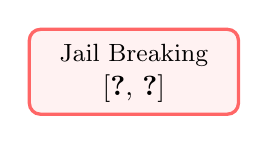
\begin{tikzpicture}[
  vuln/.style={rectangle, rounded corners, draw=red!60, fill=red!5, very thick},
  ]
 \node [vuln] (v) {
    \begin{tabular}{c}
    \makebox[2cm][c]{\small Jail Breaking} \\
    \cite{10.1007/s10515-026-00628-7,11417765}
    \end{tabular}
 };
  \end{tikzpicture} &
  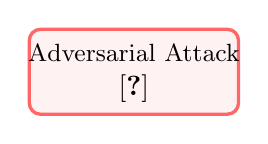
\begin{tikzpicture}[
  vuln/.style={rectangle, rounded corners, draw=red!60, fill=red!5, very thick},
  ]
 \node [vuln] (v) {
    \begin{tabular}{c}
    \makebox[2cm][c]{\small Adversarial Attack} \\
    \cite{10.1007/s10515-024-00464-7}
    \end{tabular}
 };
  \end{tikzpicture} \\
  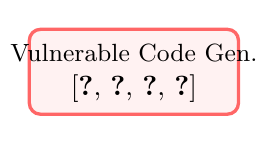
\begin{tikzpicture}[
  vuln/.style={rectangle, rounded corners, draw=red!60, fill=red!5, very thick},
  ]
 \node [vuln] (v) {
    \begin{tabular}{c}
    \makebox[2cm][c]{\small Vulnerable Code Gen.} \\
    \cite{copilotsecurity,10301242,10538871,GLAS2026104842}
    \end{tabular}
 };
  \end{tikzpicture} &
  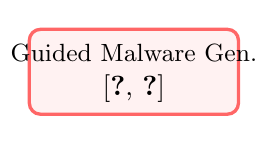
\begin{tikzpicture}[
  vuln/.style={rectangle, rounded corners, draw=red!60, fill=red!5, very thick},
  ]
 \node [vuln] (v) {
    \begin{tabular}{c}
    \makebox[2cm][c]{\small Guided Malware Gen.} \\
    \cite{ITURBE2024104077,llmbackdoordet} % improper article ID. The article leverage LLM for attacking.
    \end{tabular}
 };
  \end{tikzpicture} \\
  \multicolumn{2}{c}{
    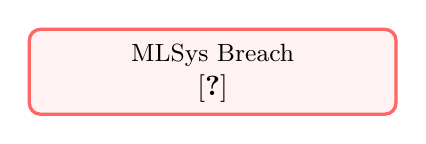
\begin{tikzpicture}[
  vuln/.style={rectangle, rounded corners, draw=red!60, fill=red!5, very thick},
  ]
 \node [vuln] (v) {
    \begin{tabular}{c}
    \makebox[4cm][c]{\small MLSys Breach} \\
    \cite{10.1145/3756681.3757083}
    \end{tabular}
 };
    \end{tikzpicture}
  } \\
\end{tabular}
};


\node[base] (harness) [right=of infer] {
  \begin{tabular}{cc}
  \multicolumn{2}{c}{\textbf{Agent Harness}} \\
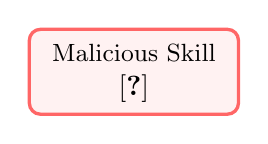
\begin{tikzpicture}[
  vuln/.style={rectangle, rounded corners, draw=red!60, fill=red!5, very thick},
  ]
 \node [vuln] (v) {
   \begin{tabular}{c}
    \makebox[2cm][c]{\small Malicious Skill} \\
    \cite{skillvulns}
   \end{tabular}
 };
  \end{tikzpicture} &
  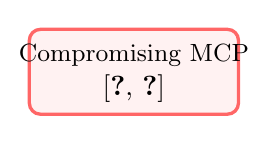
\begin{tikzpicture}[
  vuln/.style={rectangle, rounded corners, draw=red!60, fill=red!5, very thick},
  ]
 \node [vuln] (v) {
   \begin{tabular}{c}
    \makebox[2cm][c]{\small Compromising MCP} \\
    \cite{10.1145/3814959,mcpvulns}
   \end{tabular}
 };
  \end{tikzpicture} \\
  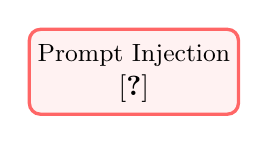
\begin{tikzpicture}[
  vuln/.style={rectangle, rounded corners, draw=red!60, fill=red!5, very thick},
  ]
 \node [vuln] (v) {
   \begin{tabular}{c}
    \makebox[2cm][c]{\small Prompt Injection} \\
    \cite{11536564}
   \end{tabular}
 };
  \end{tikzpicture} &
  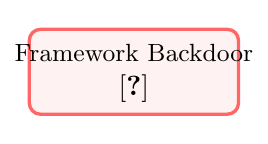
\begin{tikzpicture}[
  vuln/.style={rectangle, rounded corners, draw=red!60, fill=red!5, very thick},
  ]
 \node [vuln] (v) {
   \begin{tabular}{c}
    \makebox[2cm][c]{\small Framework Backdoor} \\
    \cite{11536564}
   \end{tabular}
 };
  \end{tikzpicture}  \\

  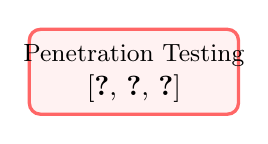
\begin{tikzpicture}[
  vuln/.style={rectangle, rounded corners, draw=red!60, fill=red!5, very thick},
  ]
 \node [vuln] (v) {
  \begin{tabular}{c}
    \makebox[2cm][c]{\small Penetration Testing} \\
    \cite{10970188,11418046,10.1145/3766895}
  \end{tabular}
 };
  \end{tikzpicture} &
  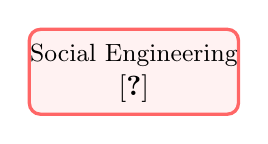
\begin{tikzpicture}[
  vuln/.style={rectangle, rounded corners, draw=red!60, fill=red!5, very thick},
  ]
 \node [vuln] (v) {
    \begin{tabular}{c}
    \makebox[2cm][c]{\small Social Engineering} \\
    \cite{10187385}
    \end{tabular}
 };
  \end{tikzpicture} 
\end{tabular}
};

\end{tikzpicture}
% \end{document}

  \caption{The vulnerabilities of an LLM in \textit{Training}, \textit{Inference},
  and \textit{Agent} stage. \\
   {\small Each citation in this figure represents an attack made by a previous research.}
  }
  \label{fig:llmrisk}
\end{figure}

\subsection{Implications of Training Stage Vulnerabilities}
In its training and fine-tuning process, Large Language Models
are susceptible to \textit{data poisoning} and \textit{backdoor injection}
attacks. Speaking of Code Language Models (CLMs), its training data
may be contaminated by malicious or vulnerable code snippets.
Consequently, in their inference stage, the generated code contains
similar patterns of vulnerability or malice; certain LLM-based
bug detector may suffer reduced effectiveness. As an increasing proportion
of code is written by CLMs, \textit{data poisoning} is capable of
polluting Software Supply Chain with problematic software packages.
For instance, M. Jahanshahi et al. made a large scale investigation
into the use of Open Source Software in LLM training, and observed
a drop in vulnerability rate when the LLM is trained with "cleaner"
code (e.g. whose CVEs are resolved) \citep{11028470}. Such observations
calls for data poisoning mitigation techniques (e.g. \citep{11344010}) to 
sanitize the defects in the training data.

% SSC attack vector 1.
\par Researchers have noticed the existence of \textit{backdoor}s in
these CLMs, which enabled the attacker to manipulate a model's response
with a trigger in the prompt to obtain malicious code from the model's
output \citep{li2021backdoorattackspretrainedmodels}. 
Y. Qu et al. conducted a review of LLM backdoor attacks, 
fine-tuning based  methods, and
applications (including deliberate malicious code injection)
\citep{10.1016/j.infsof.2025.107707}. Like \textit{data poisoning},
\textit{backdoor attack} can also inject malicious package into
Software Supply Chain.





% Closing this study.
\section{Conclusions}\label{sec:conclude}

\par Software Supply Chain is a crucial infrastructure of
our digitalized world. It is nevertheless susceptible to 
vulnerable/malicious code, compromised build infrastructures,
and targeted human developers. To this end, a wide variety of
LLM-based defense techniques have been proposed, where LLMs
are leveraged because of their capabilities of contextual
reasoning and code comprehension.
However, the sheer number of SSC attacks in recent years
calls for more effective defense methods.

\par This study also delves into LLM's employment for attacking
purposes. Through a rigorous analysis of collected 23 "LLM for SSC attack"
studies presented in RQ3 (Section~\ref{sec:rq3}), we conclude that
LLMs are capable of assisting attackers in breaching SSC
via vulnerable code injection or social engineering attack.

\paragraph*{Calls for ethical use of LLMs in software development}
Based on our literature review and analysis, we suggest the following
mitigation and counter-measures:

\begin{itemize}
  \item \textit{Software Developers} (Users Code Language Models) 
  should be aware of the LLM's
  tendency in providing seemingly correct code with subtle
  bugs, vulnerabilities, or even malicious code. Therefore,
  rigorous code-review and state-of-the-art linter are recommended.
  Nevertheless, the use of LLM in reporting software vulnerabilities
  must be followed by thorough investigation of veteran developers
  in case of inaccurate content.

 \item \textit{LLM providers} should be cautions of data poisoning
 attacks and low-quality training data, so that the safety of LLM-generated
  code can be improved. Furthermore, ethical alignment of LLMs
  should be implemented to counter jailbreaking or prompt injection
  attacks. 

  \item \textit{Package Managers} and \textit{Code Hosting Platforms}
  should enhance scrutiny and governance of published software packages, possibly
  employing state-of-the-art threat detectors in case of potential
  attacks from malicious code or severe vulnerabilities.
\end{itemize}


\bibliography{main}
\end{document}

